\subsubsection*{ROS2}
\begin{frame}
     \frametitle{ROS 2 : Fonctionnement}
        \begin{itemize}
            \item \textbf{ROS} (Robot Operating System) est un framework qui facilite la communication entre les composants d'un robot (capteurs, actionneurs, etc.).
            %\item L'architecture est basée sur des \textbf{nœuds} (programmes) qui communiquent via des \textbf{topics} (canaux).
            %\item Ce système utilise un modèle \textbf{publisher-subscriber} : un nœud publie des données sur un topic, et un autre y souscrit pour les recevoir.
        \end{itemize}

        \begin{figure}
            \centering
            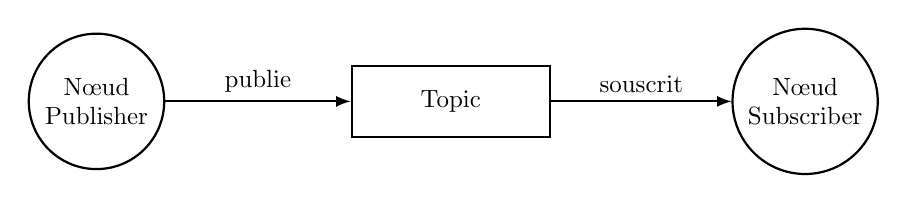
\begin{tikzpicture}[scale=0.9, transform shape, >=latex]
                \tikzset{
                    rosnode/.style={circle, draw, thick, minimum size=14mm, align=center},
                    topic/.style={rectangle, draw, thick, minimum width=28mm, minimum height=10mm, align=center}
                }
                \node[rosnode] (pub) at (0,0) {Nœud\\Publisher};
                \node[topic]   (top) at (5,0) {Topic};
                \node[rosnode] (sub) at (10,0) {Nœud\\Subscriber};
                \draw[->, thick] (pub) -- node[above, midway]{publie} (top);
                \draw[->, thick] (top) -- node[above, midway]{souscrit} (sub);
            \end{tikzpicture}
            \caption{Communication publisher-subscriber via un topic.}
            \label{fig:ros2_topic}
        \end{figure}
    \end{frame}